
% This LaTeX was auto-generated from an M-file by MATLAB.
% To make changes, update the M-file and republish this document.

\documentclass{article}
\usepackage{graphicx}
\usepackage{color}

\sloppy
\definecolor{lightgray}{gray}{0.5}
\setlength{\parindent}{10pt}
\usepackage[margin=1in]{geometry}

\begin{document}

\title{Dynamical Adaptation in ORNs}
\author{Srinivas Gorur-Shandilya}
\maketitle

    
    
\section*{Fitting Damon's Model to ORN Data}

\begin{par}
In this document, I will try to fit the Dynamical Adaptaiton (DA) model to data. The Dynamical Adaptaiton model has 8 parameters that need to be constrained. Setting one of them, $\tau_{r}$, to zero eliminates the need to solve a differential equation, and the response is given in closed form as a funciton of the stimulus. This greatly speeds up code execution. We also constrain $n_{y}$ and $n_{z}$ to default values of 2.
\end{par} \vspace{1em}

\subsection*{Contents}

\begin{itemize}
\setlength{\itemsep}{-1ex}
   \item Fitting DA Model to synthetic data
   \item Fitting DA Model to real data
   \item Real Data: Gain Analysis
\end{itemize}


\subsection*{Fitting DA Model to synthetic data}

\begin{par}
Fitting these 7 parameters to data is a hard problem. First, I will try to fit these 7 parameters to synthetic data, generated by the DA model. We generate some synthetic stimulus using random noise inputs filtered by some low pass function (see top panel in plot below).
\end{par} \vspace{1em}

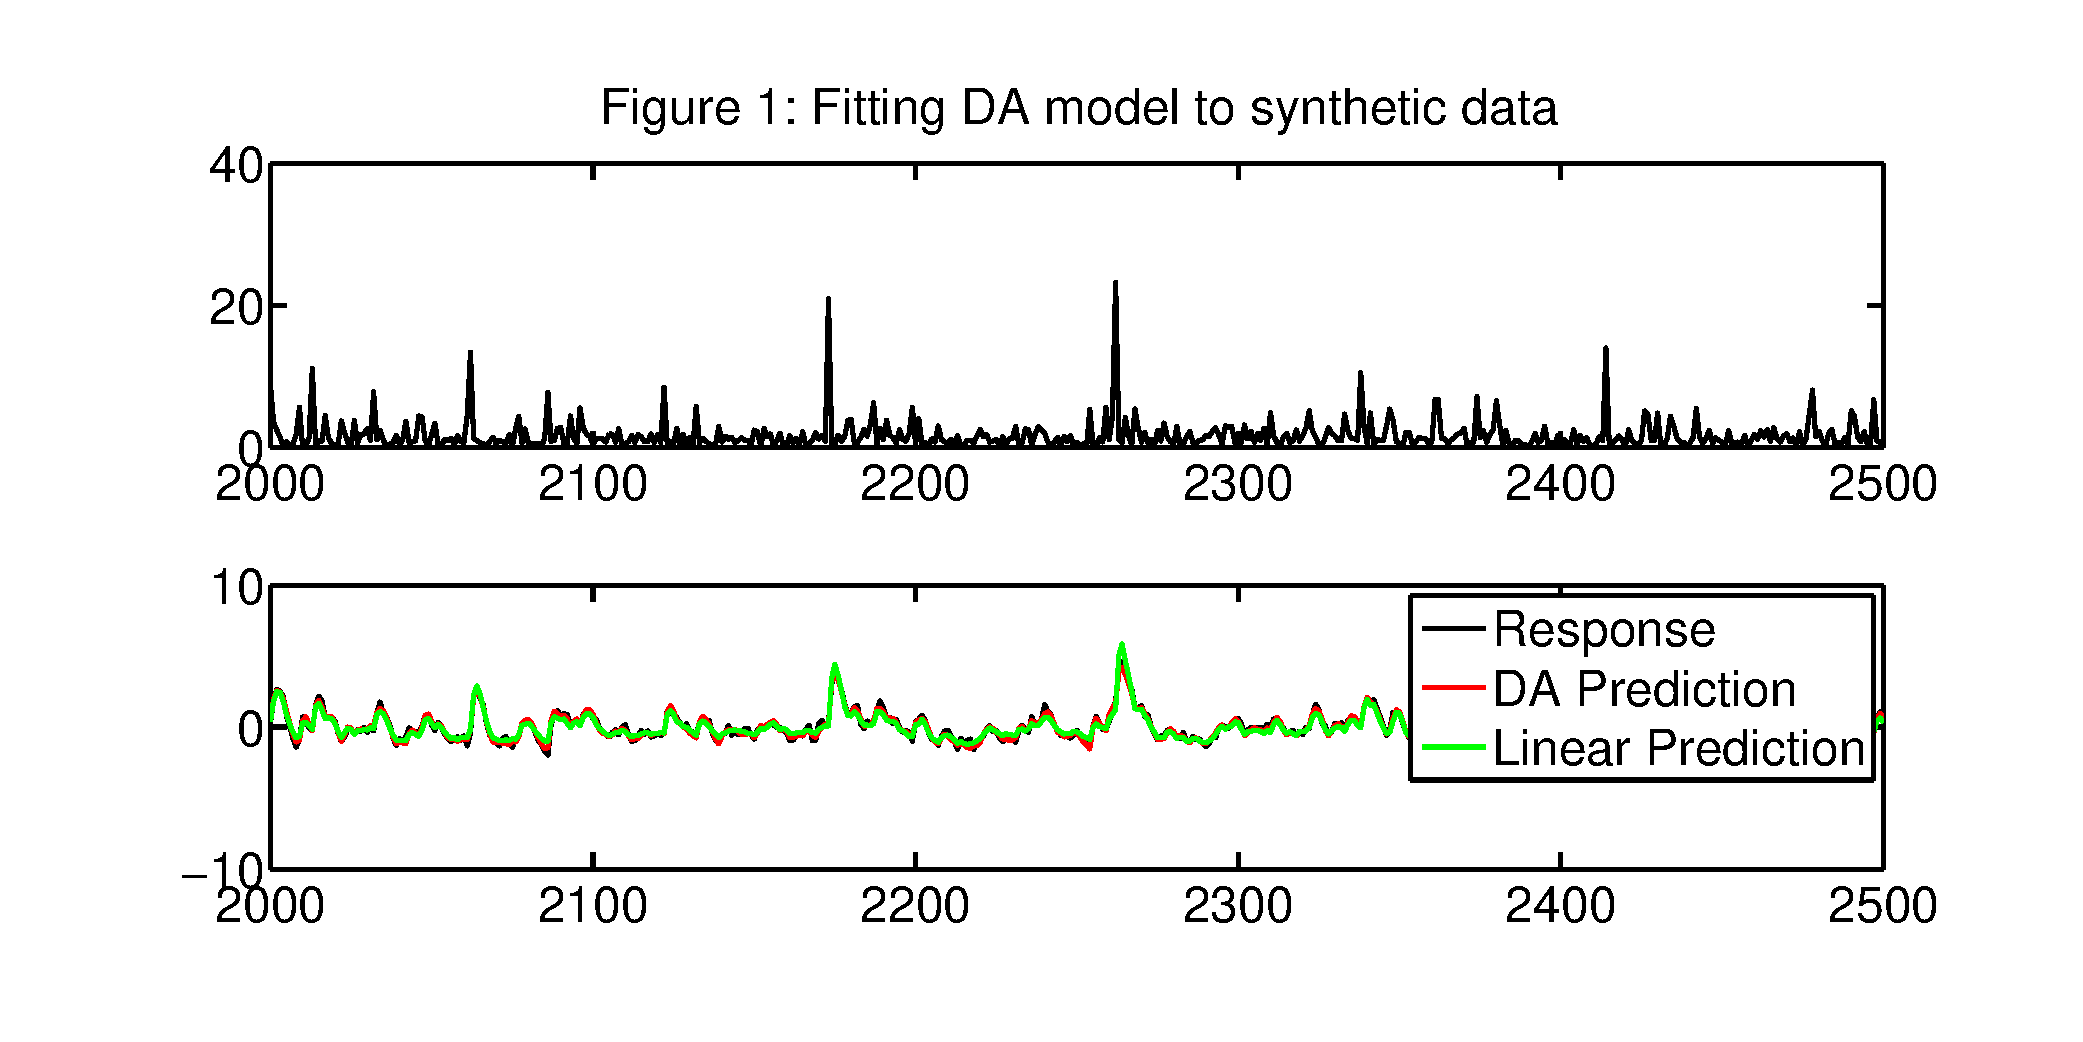
\includegraphics [width=\textwidth]{FittingDAModel_01.pdf}
\begin{par}
Then, choosing some arbitrary parameters for the DA model, we generate the DA model output. This is shown in the black line in the figure below (the bottom panel). Using this model output and the known input, we run a global optimisation procedure (a genetic algorithm) on this data set fifty times, and estimate the parameters that give predicted responses with lowest least square error. One such solution is shown below in red, together with a simple linear prediction from a linear filter in green.
\end{par} \vspace{1em}
\begin{par}
OK, so the genetic algorithm seems to find some parameters that do an OK job of predicting the response. How good is the estimate of the parameters of the model itself? In the following figure I plot the ensemble predictions from the 50 different realisations of the optimisation algorithm, normalised by the value of each parameter to visualse how well we can estimate the "real" parameters of the model.
\end{par} \vspace{1em}

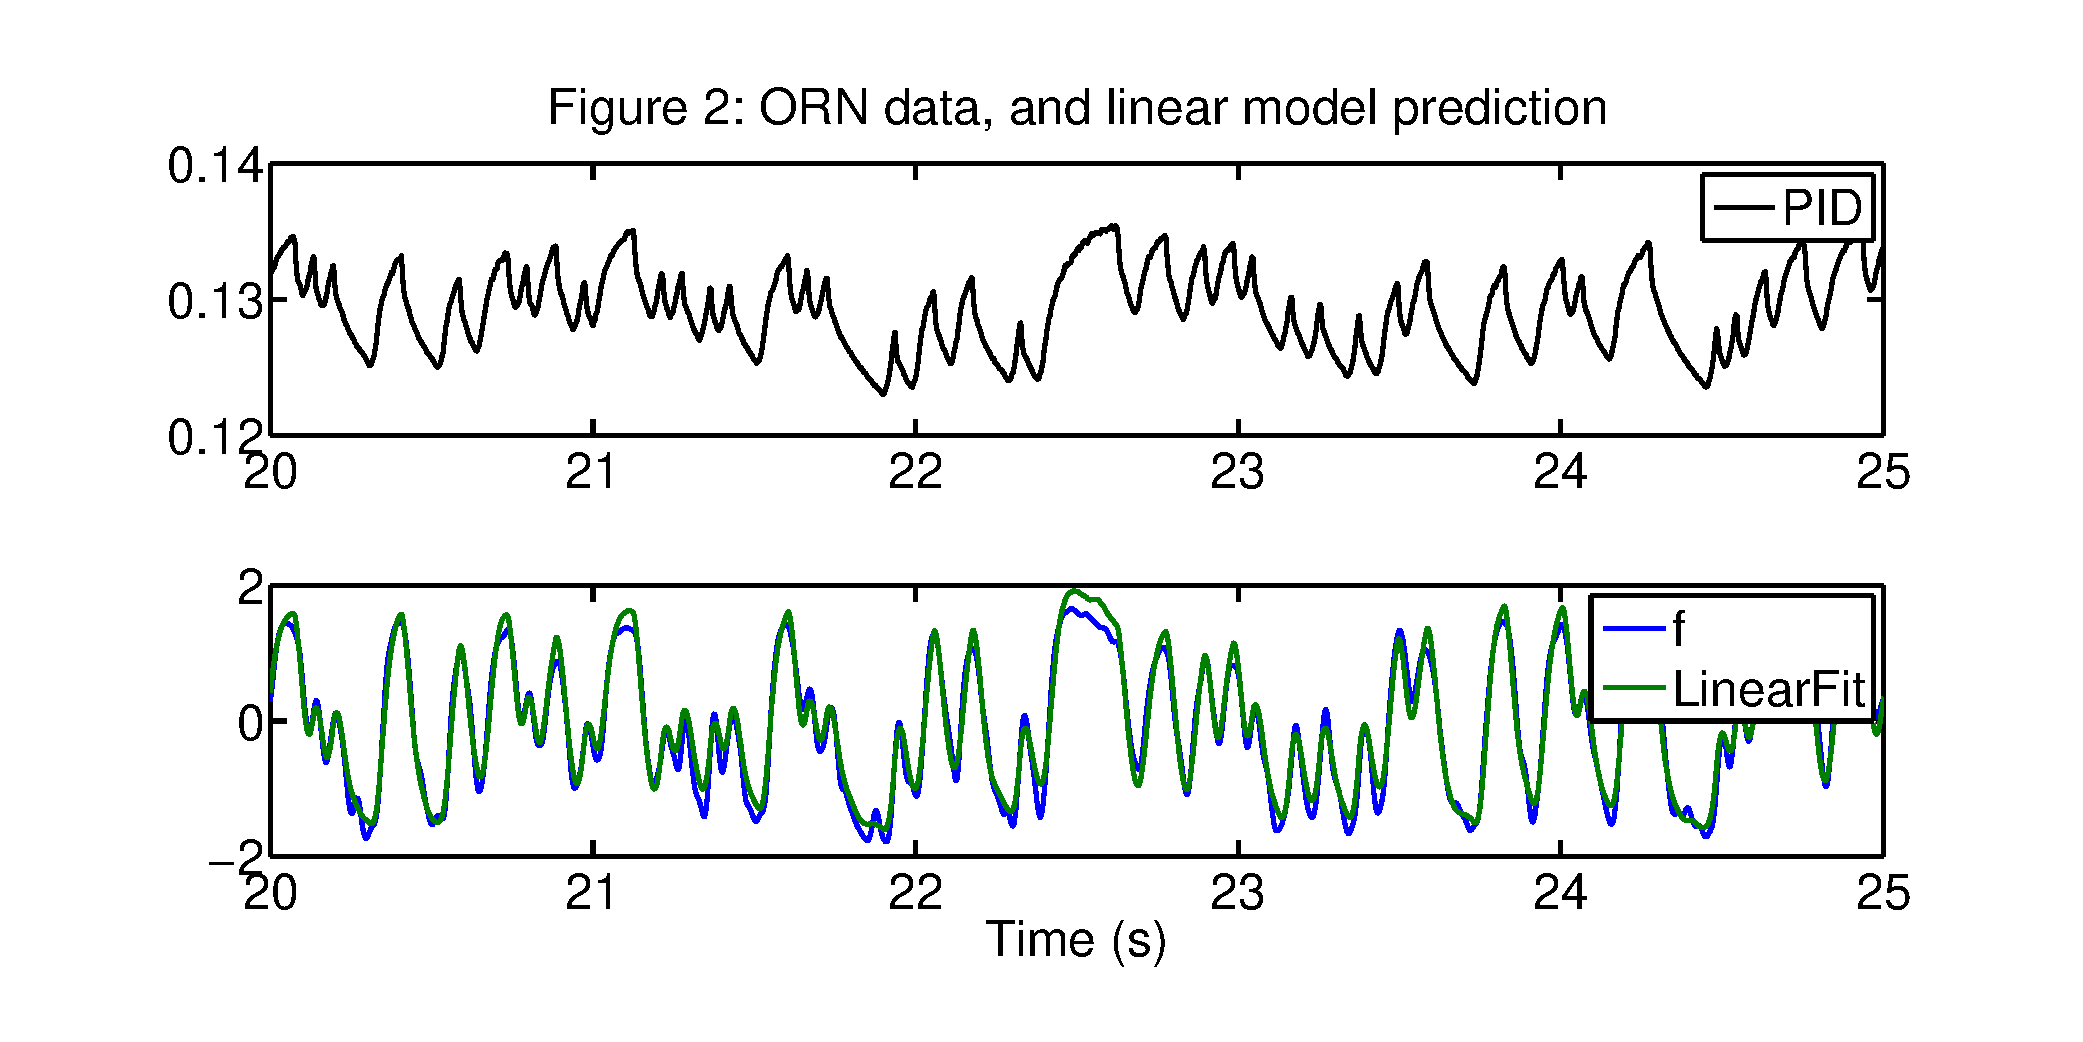
\includegraphics [width=\textwidth]{FittingDAModel_02.pdf}
\begin{par}
That's quite a spread. To understand whether this spread is because our optimisation algorithm is fundamentally flawed, or to see if the mapping from the space of model parameters to model output is many to one, we plot the r-square of predicted response vs. the absolute error of the prediction of the model parameters. In this plot, each color is a different parameter, and the colors correspond to colors in previous plots.
\end{par} \vspace{1em}
\begin{par}
Ignoring for the moment the fact that there are two clusters, and concentrating only on the better-fit cluster (the one on the right), we see no correlation between quality of fit (as measured by r-square) and the relative absolute difference between estimated parameter and actual parameter of the DA model.
\end{par} \vspace{1em}

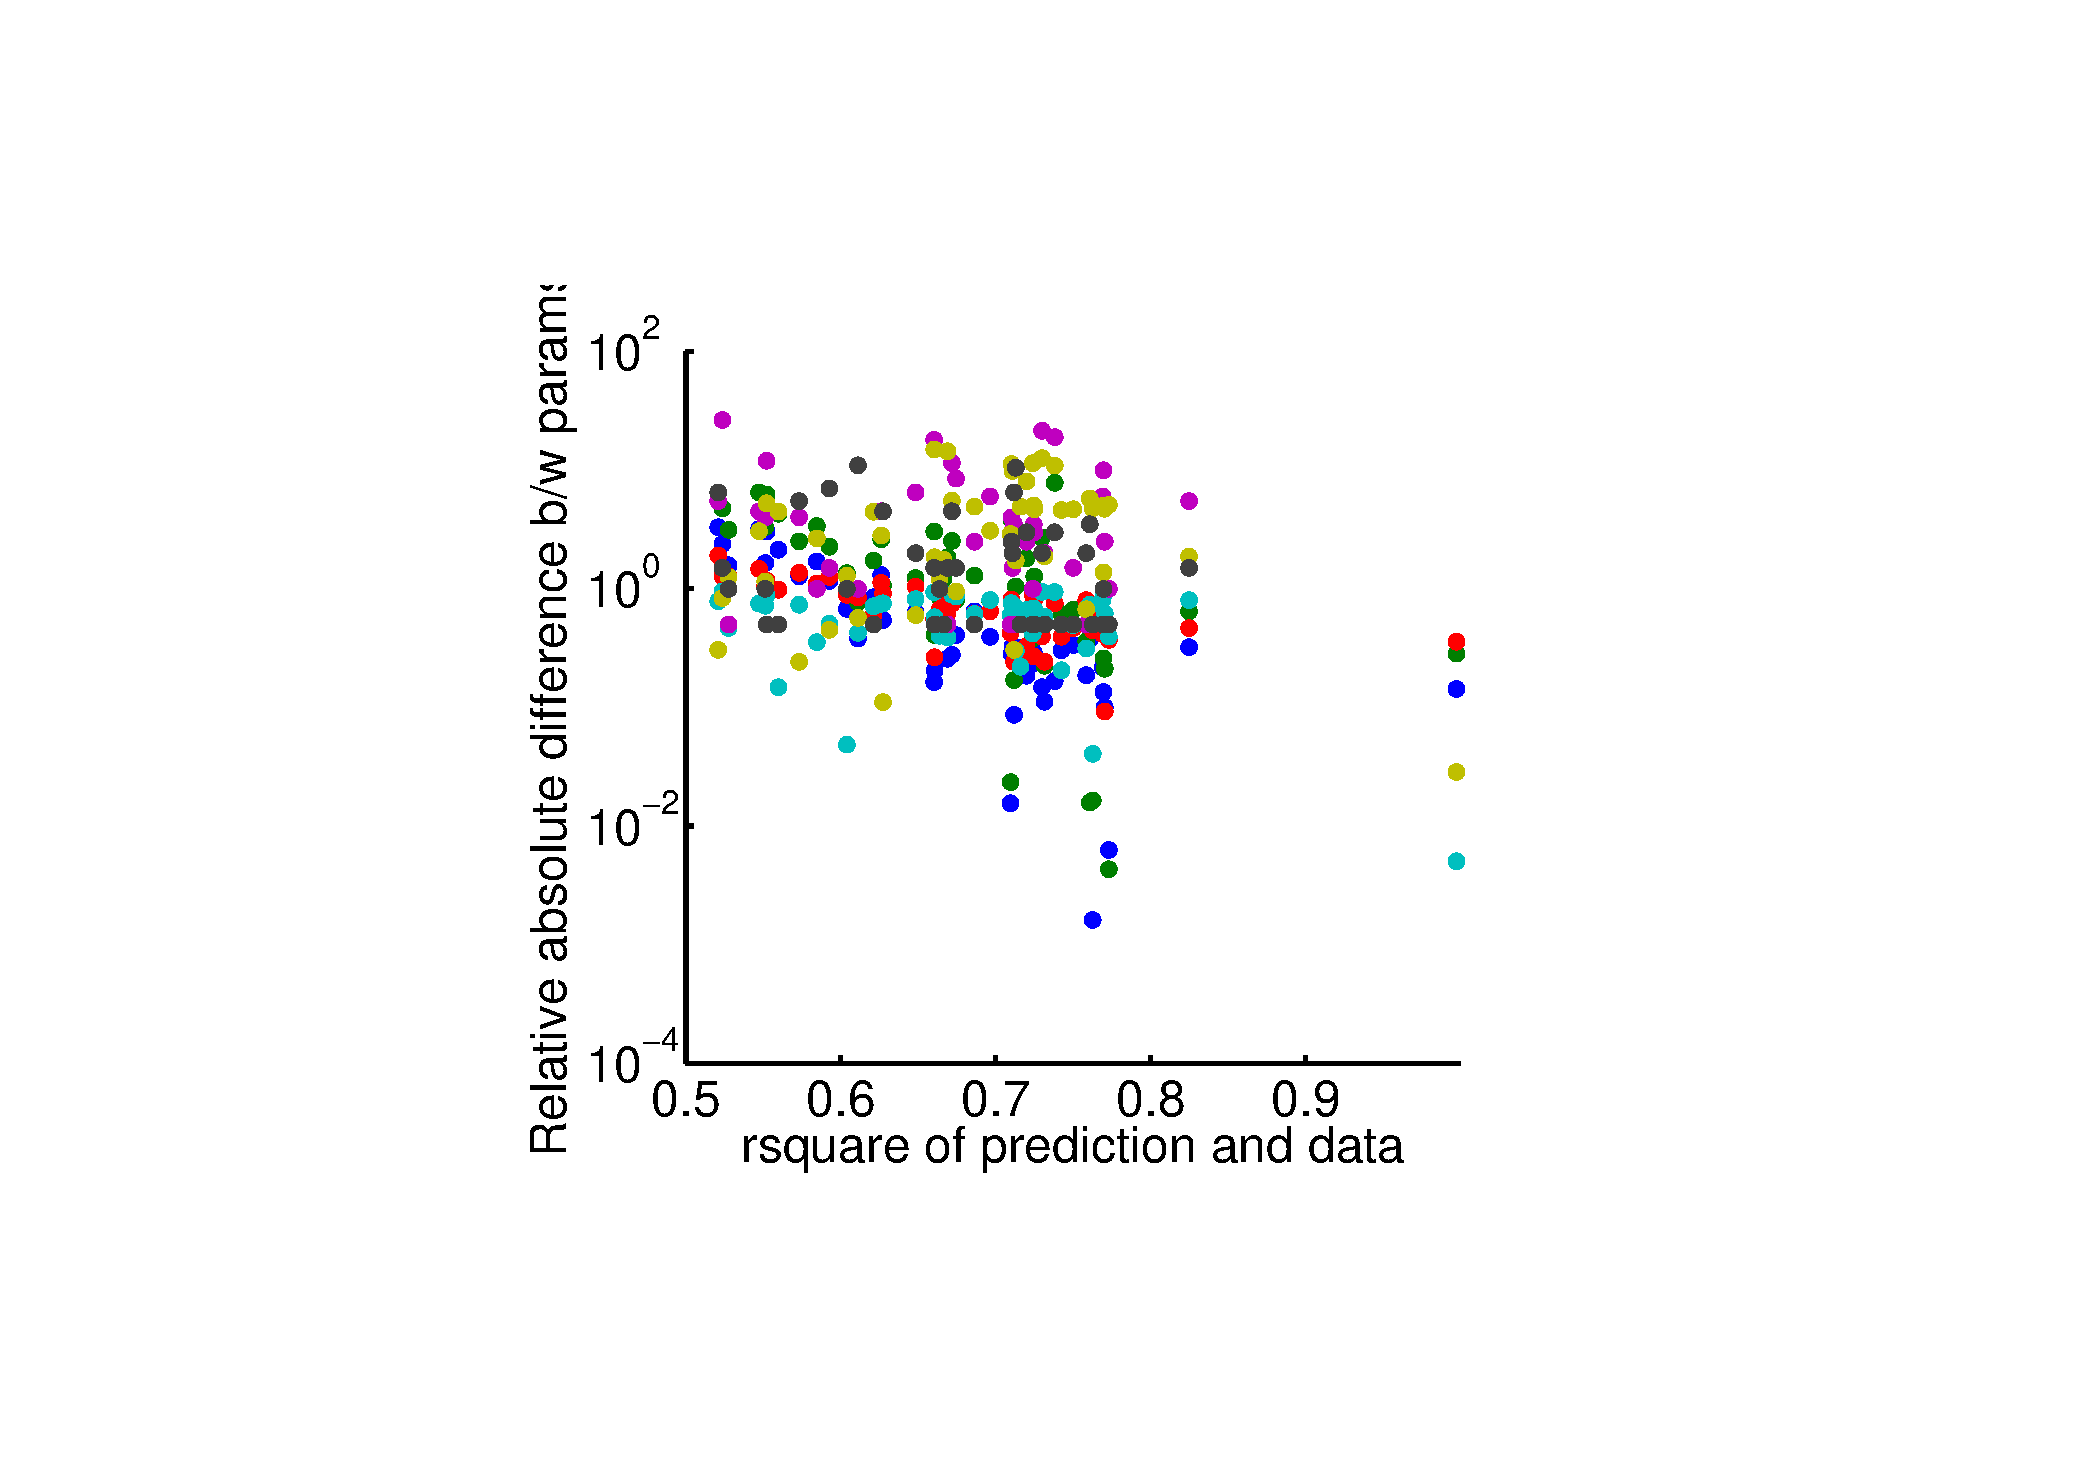
\includegraphics [width=\textwidth]{FittingDAModel_03.pdf}


\subsection*{Fitting DA Model to real data}

\begin{par}
Now we understand how the fitting works, we will try to fit real data. The following figure shows the sample data we use. The top panel shows the stimulus as measured by the PID, and the bottom panel shows the real firing rate of the ORN. Both the PID and the ORN firing rate have been rescaled so that they range from [0,1].
\end{par} \vspace{1em}

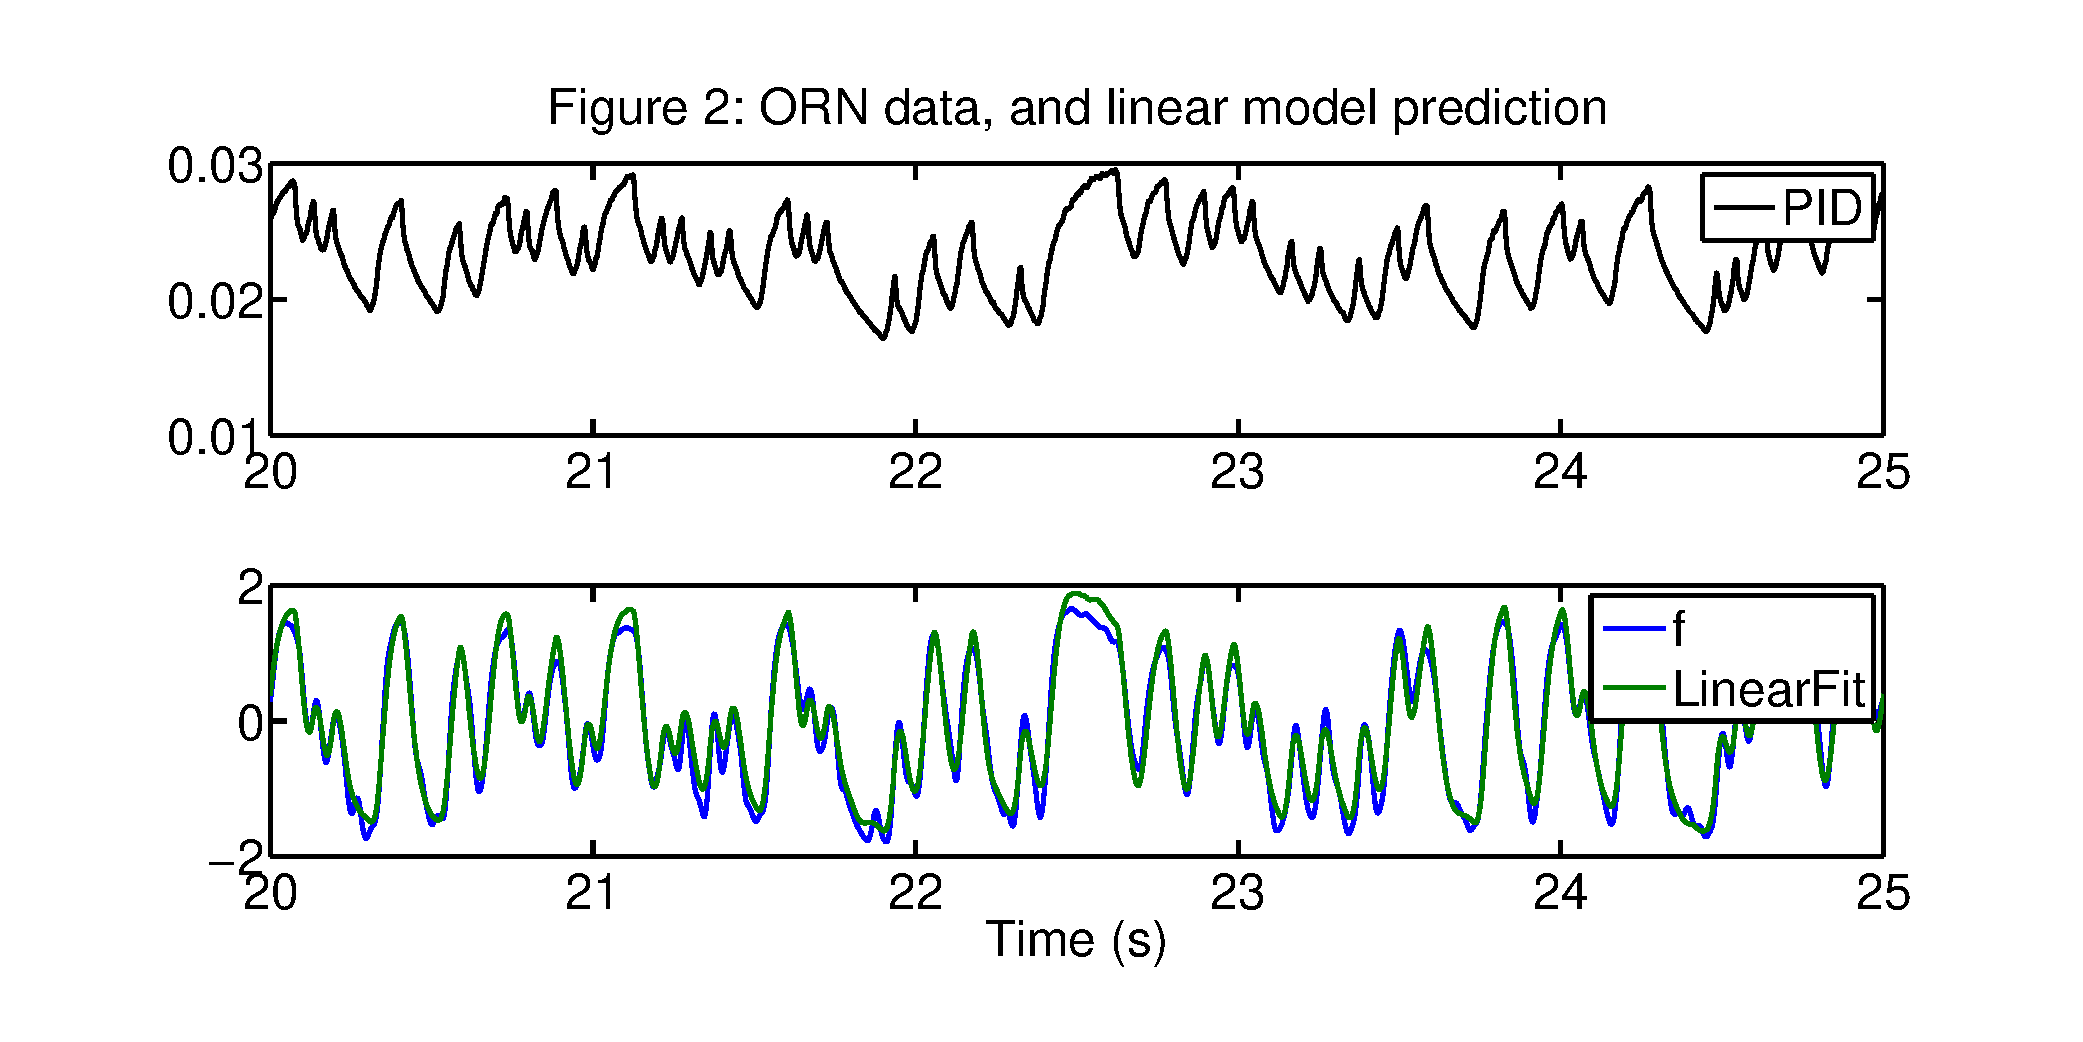
\includegraphics [width=\textwidth]{FittingDAModel_04.pdf}

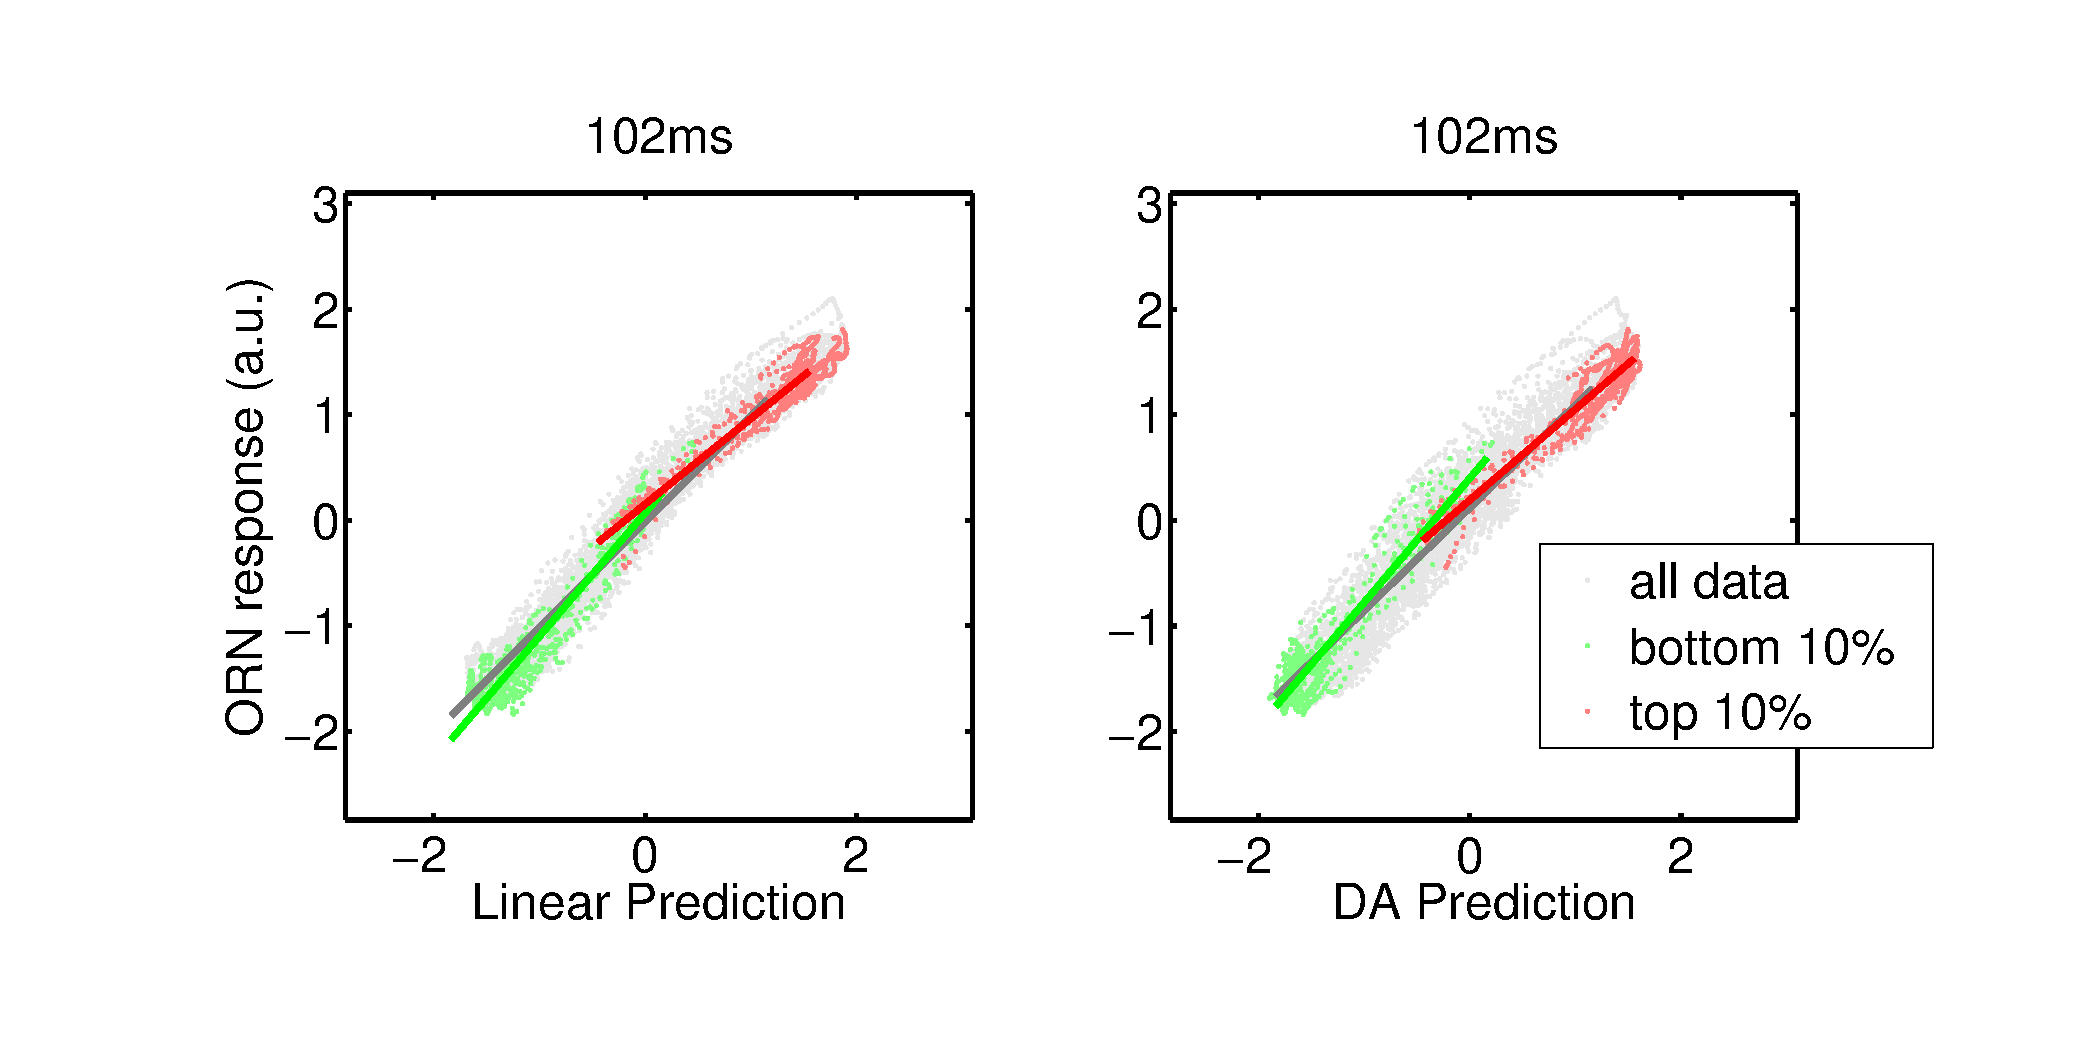
\includegraphics [width=\textwidth]{FittingDAModel_05.pdf}
\begin{par}
No we try to fit the DA model to this data, as before.
\end{par} \vspace{1em}

        \color{lightgray} \begin{verbatim}Starting parallel pool (parpool) using the 'local' profile ... connected to 4 workers.
\end{verbatim} \color{black}
    
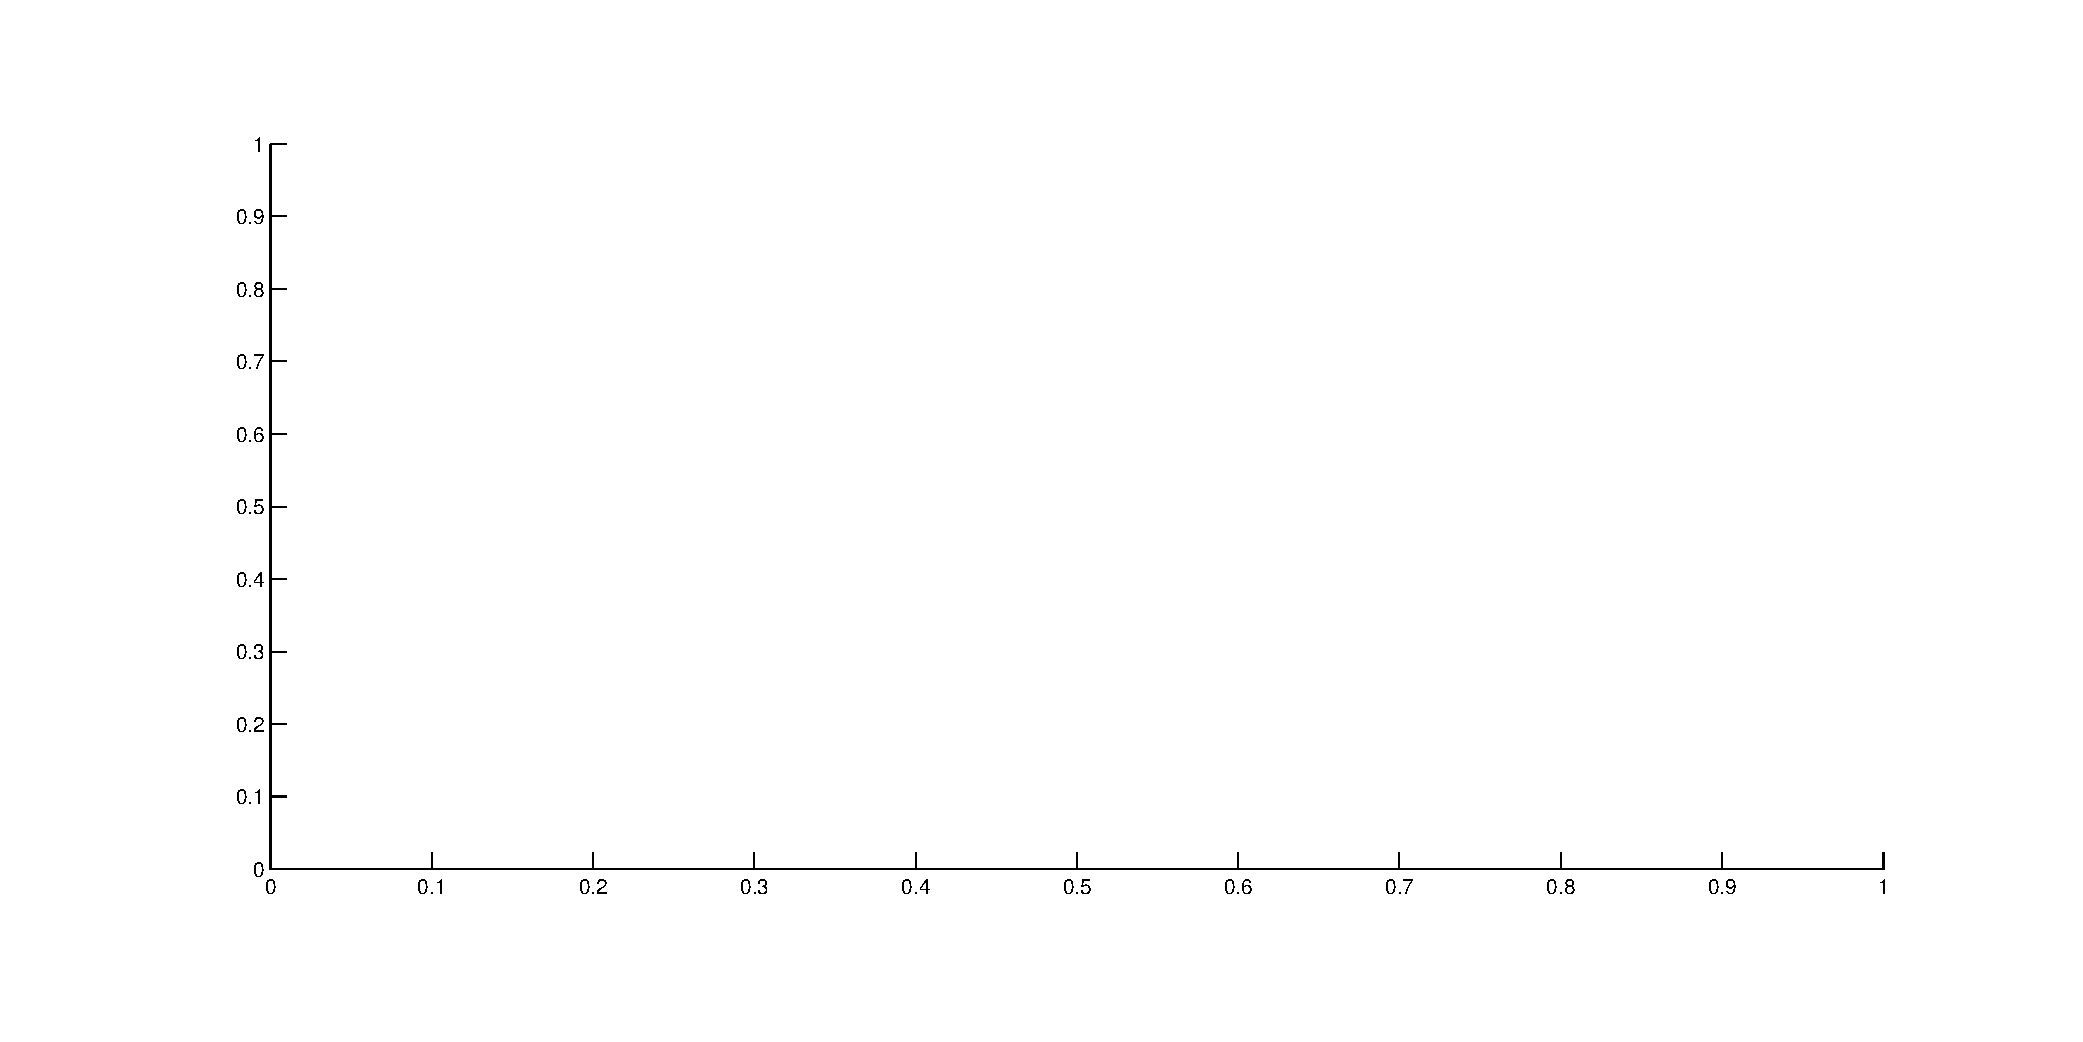
\includegraphics [width=\textwidth]{FittingDAModel_06.pdf}

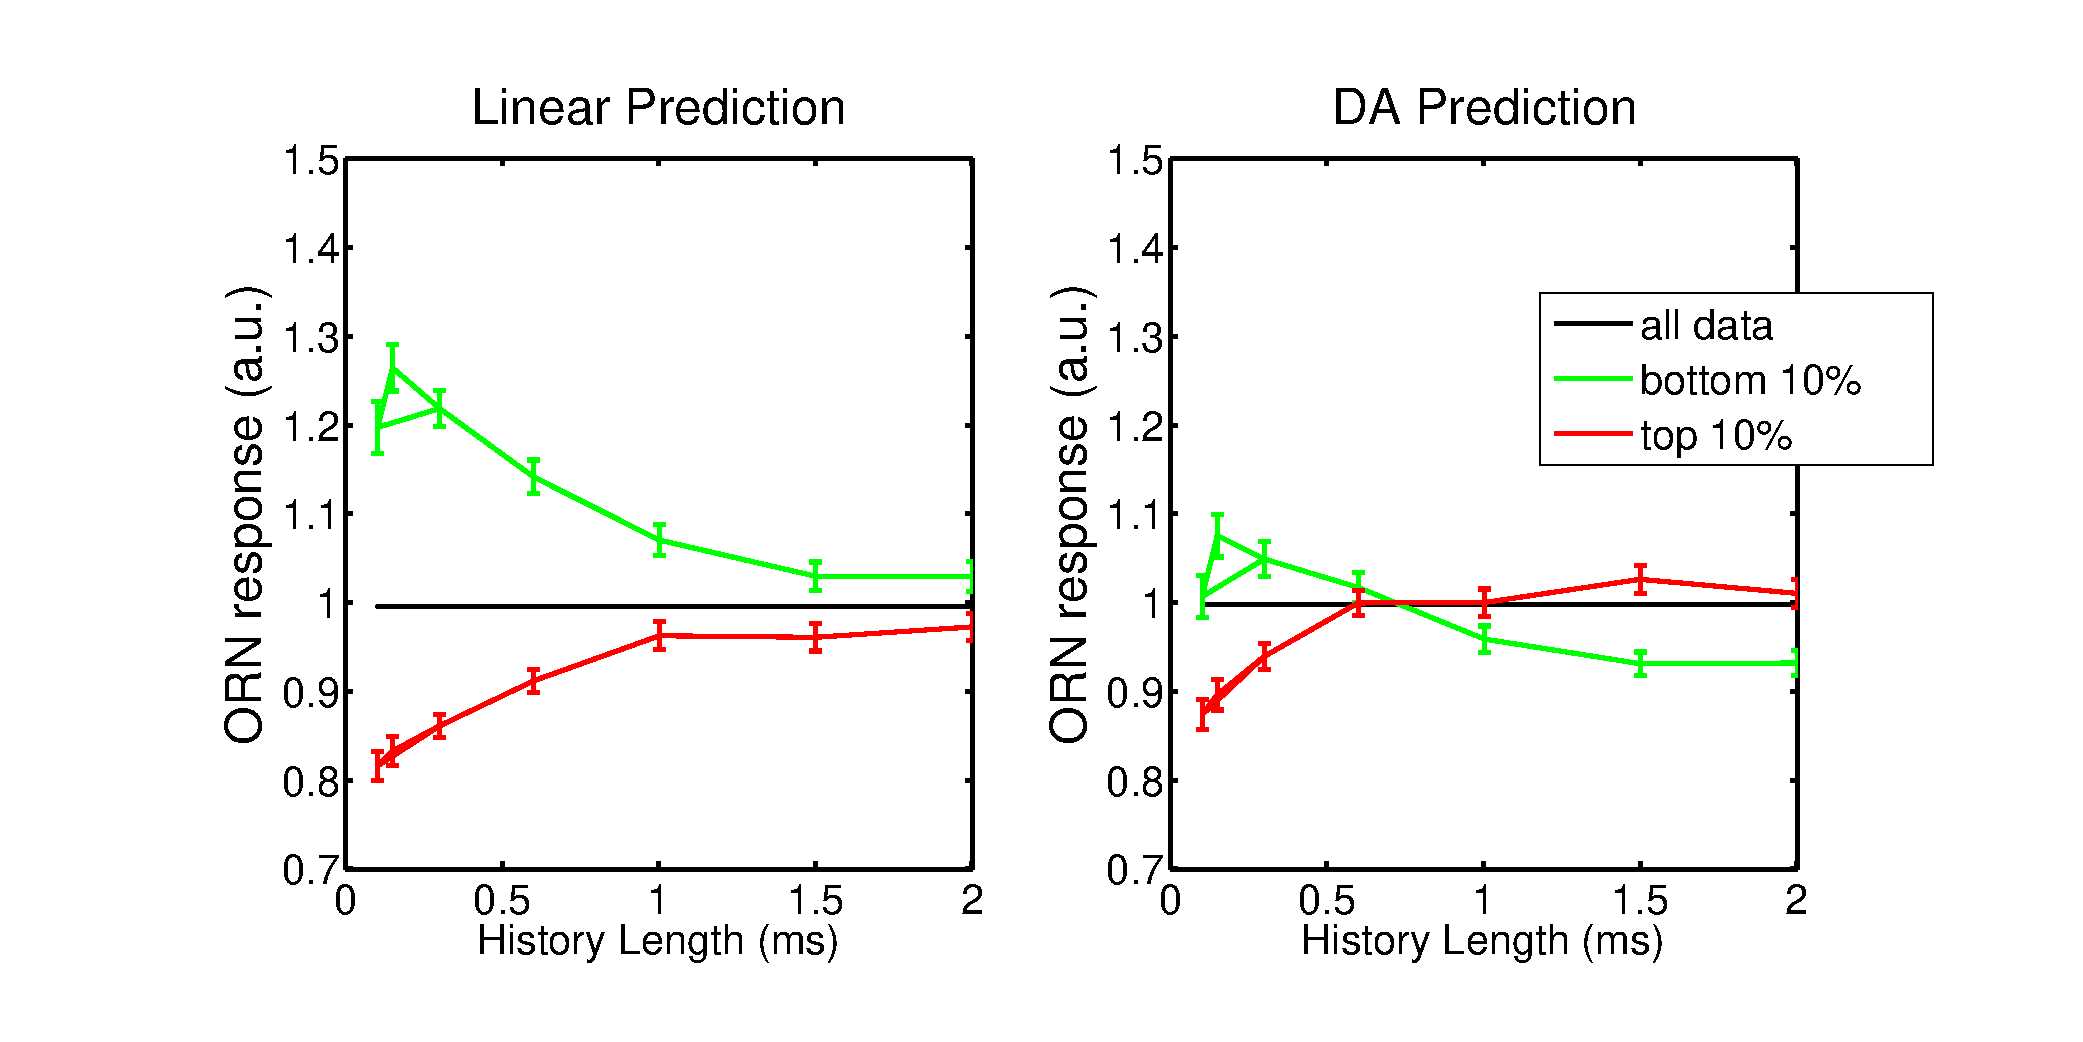
\includegraphics [width=\textwidth]{FittingDAModel_07.pdf}
\begin{par}
This is horrible. I don't know why the fit doesn't work. Instead, I'm going to try fitting to the valve signal and see if that works.
\end{par} \vspace{1em}

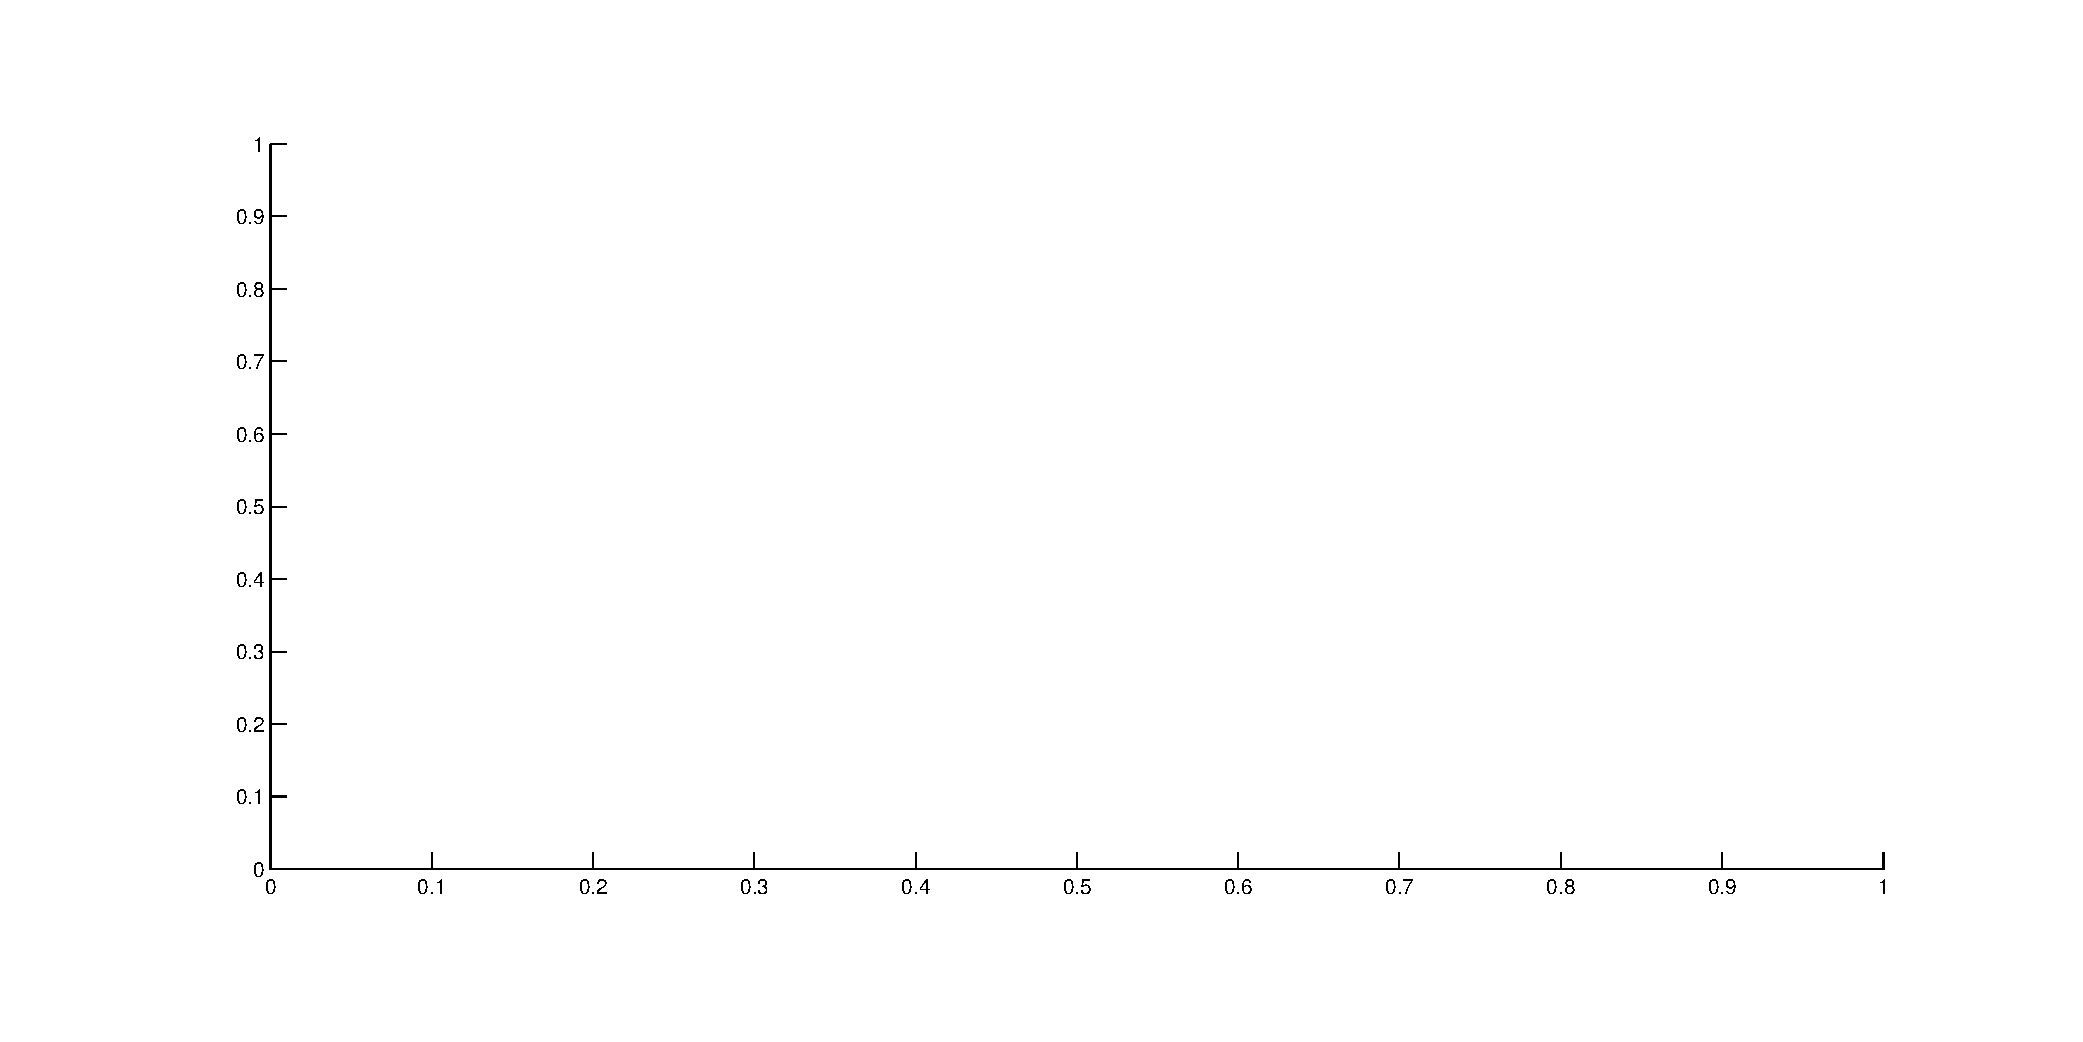
\includegraphics [width=\textwidth]{FittingDAModel_08.pdf}

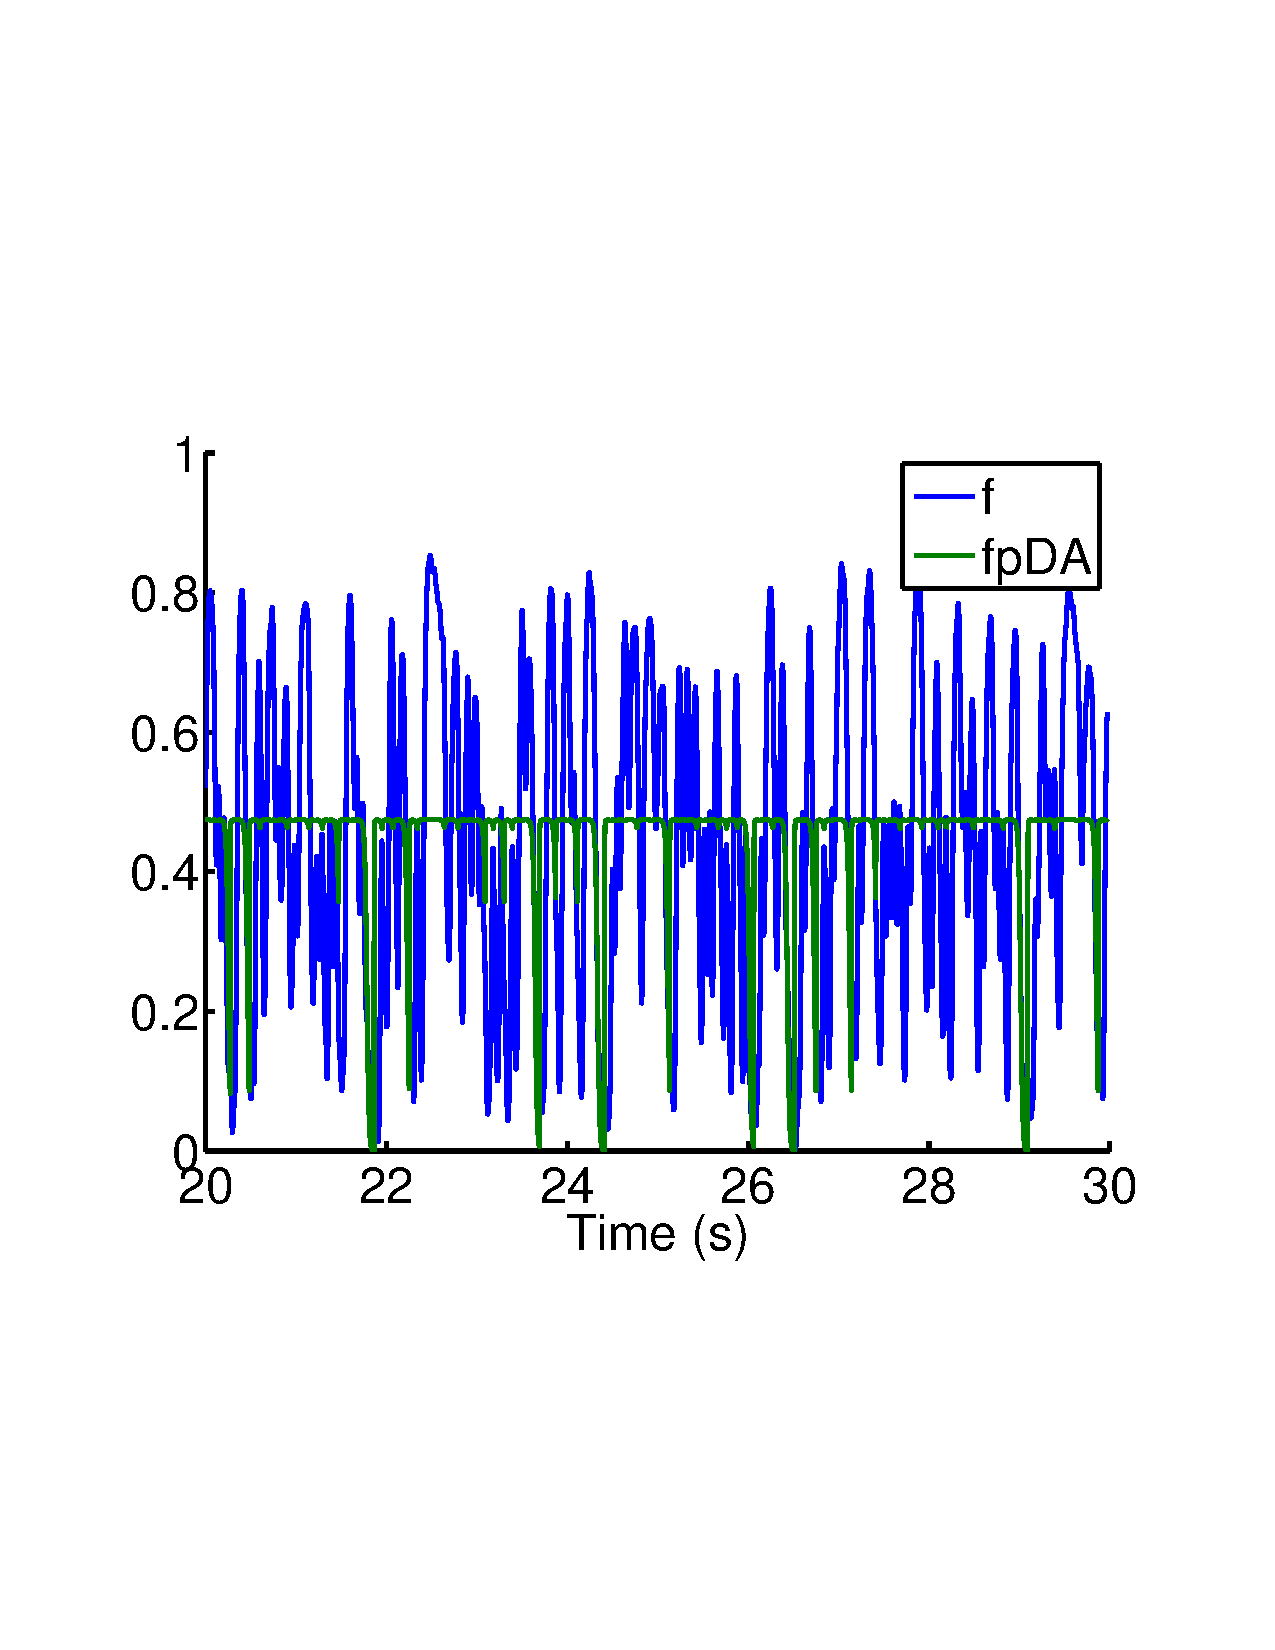
\includegraphics [width=\textwidth]{FittingDAModel_09.pdf}


\subsection*{Real Data: Gain Analysis}




\end{document}
    
